\documentclass[aspectratio=169]{beamer}

\mode<presentation>
{
  \usetheme{default}
  \usecolortheme{default}
  \usefonttheme{default}
  \setbeamertemplate{navigation symbols}{}
  \setbeamertemplate{caption}[numbered]
  \setbeamertemplate{footline}[frame number]  % or "page number"
  \setbeamercolor{frametitle}{fg=white}
  \setbeamercolor{footline}{fg=black}
} 

\usepackage[english]{babel}
\usepackage[utf8x]{inputenc}
\usepackage{tikz}
\usepackage{courier}
\usepackage{array}
\usepackage{bold-extra}
\usepackage{minted}
\usepackage{ulem}
\usepackage[thicklines]{cancel}

\xdefinecolor{dianablue}{rgb}{0.18,0.24,0.31}
\xdefinecolor{darkblue}{rgb}{0.1,0.1,0.7}
\xdefinecolor{darkgreen}{rgb}{0,0.5,0}
\xdefinecolor{darkgrey}{rgb}{0.35,0.35,0.35}
\xdefinecolor{darkorange}{rgb}{0.8,0.5,0}
\xdefinecolor{darkred}{rgb}{0.7,0,0}
\definecolor{darkgreen}{rgb}{0,0.6,0}
\definecolor{mauve}{rgb}{0.58,0,0.82}

\title[2018-06-04-scipyeco-hats]{Scientific Python Ecosystem HATS}
\author{Jim Pivarski}
\institute{Princeton University -- DIANA-HEP}
\date{June 4, 2018}

\begin{document}

\logo{\pgfputat{\pgfxy(0.11, 7.4)}{\pgfbox[right,base]{\tikz{\filldraw[fill=dianablue, draw=none] (0 cm, 0 cm) rectangle (50 cm, 1 cm);}\mbox{\hspace{-8 cm}
\includegraphics[height=1 cm]{princeton-logo-long.png}
\includegraphics[height=1 cm]{diana-hep-logo-long.png}}}}}

\begin{frame}
  \titlepage
\end{frame}

\logo{\pgfputat{\pgfxy(0.11, 7.4)}{\pgfbox[right,base]{\tikz{\filldraw[fill=dianablue, draw=none] (0 cm, 0 cm) rectangle (50 cm, 1 cm);}\mbox{\hspace{-8 cm}
\includegraphics[height=1 cm]{princeton-logo.png}
\includegraphics[height=1 cm]{diana-hep-logo.png}}}}}

% Uncomment these lines for an automatically generated outline.
%\begin{frame}{Outline}
%  \tableofcontents
%\end{frame}

% START START START START START START START START START START START START START

\begin{frame}{}
\begin{center}
\LARGE \textcolor{darkblue}{Big Data: we're not the only ones anymore}
\end{center}
\end{frame}

\begin{frame}{{200~PB is a lot of data}\only<2>{, but for Amazon, it's two 18-wheelers}}
\vspace{0.35 cm}
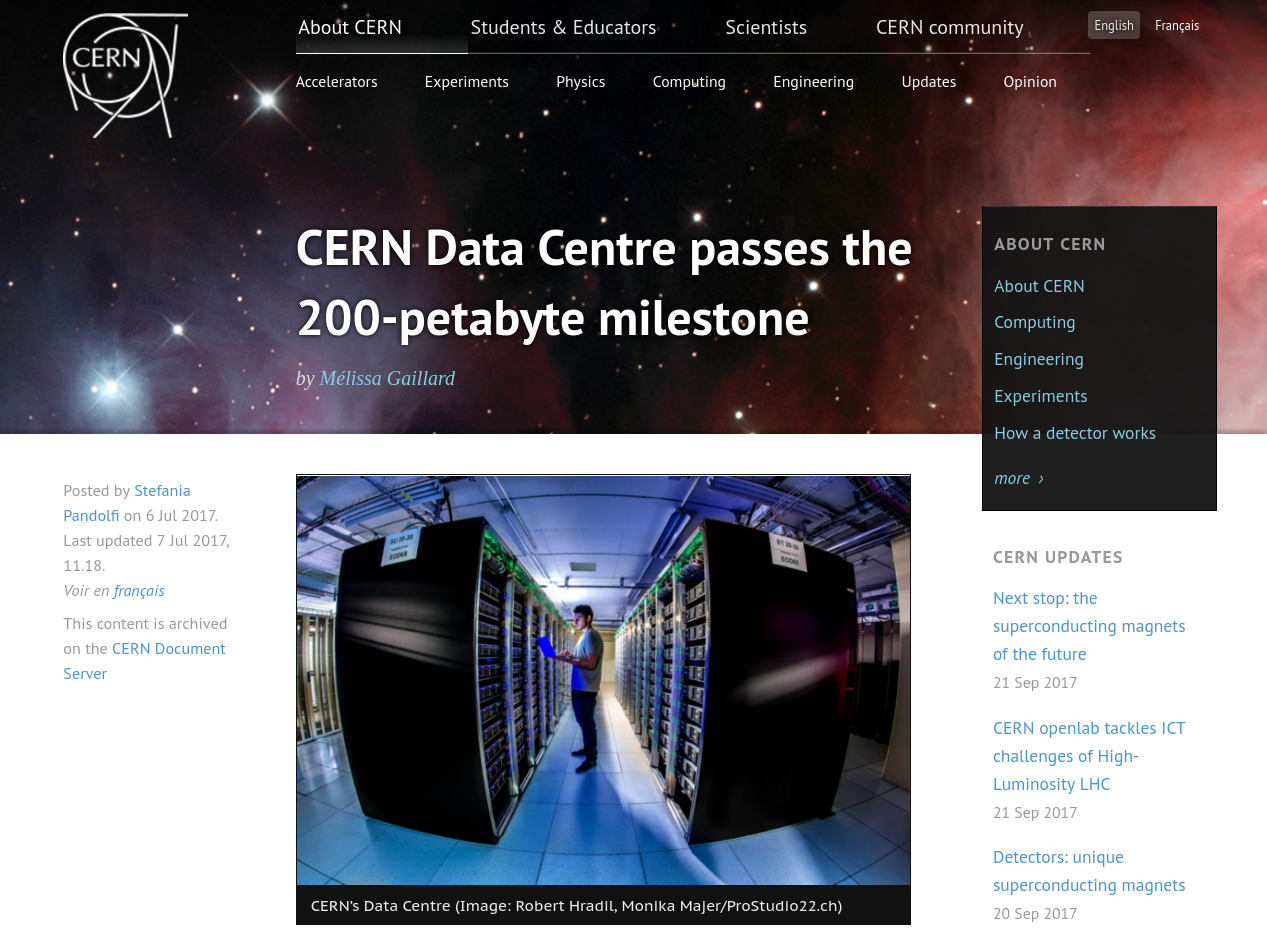
\includegraphics[width=0.73\linewidth]{cern-200pb.png}

\vspace{-4.8 cm}
\uncover<2->{\mbox{ } \hfill 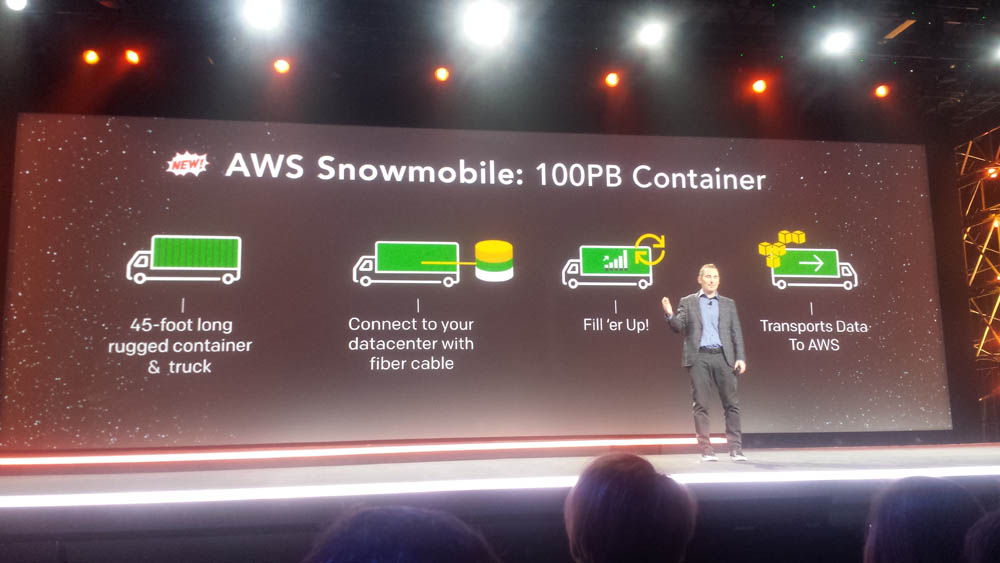
\includegraphics[width=0.7\linewidth]{aws-snowmobile.jpg}\hspace{-1 cm}}
\end{frame}

\begin{frame}{Data analysis software developed on both sides; hard to connect}
\vspace{0.17 cm}
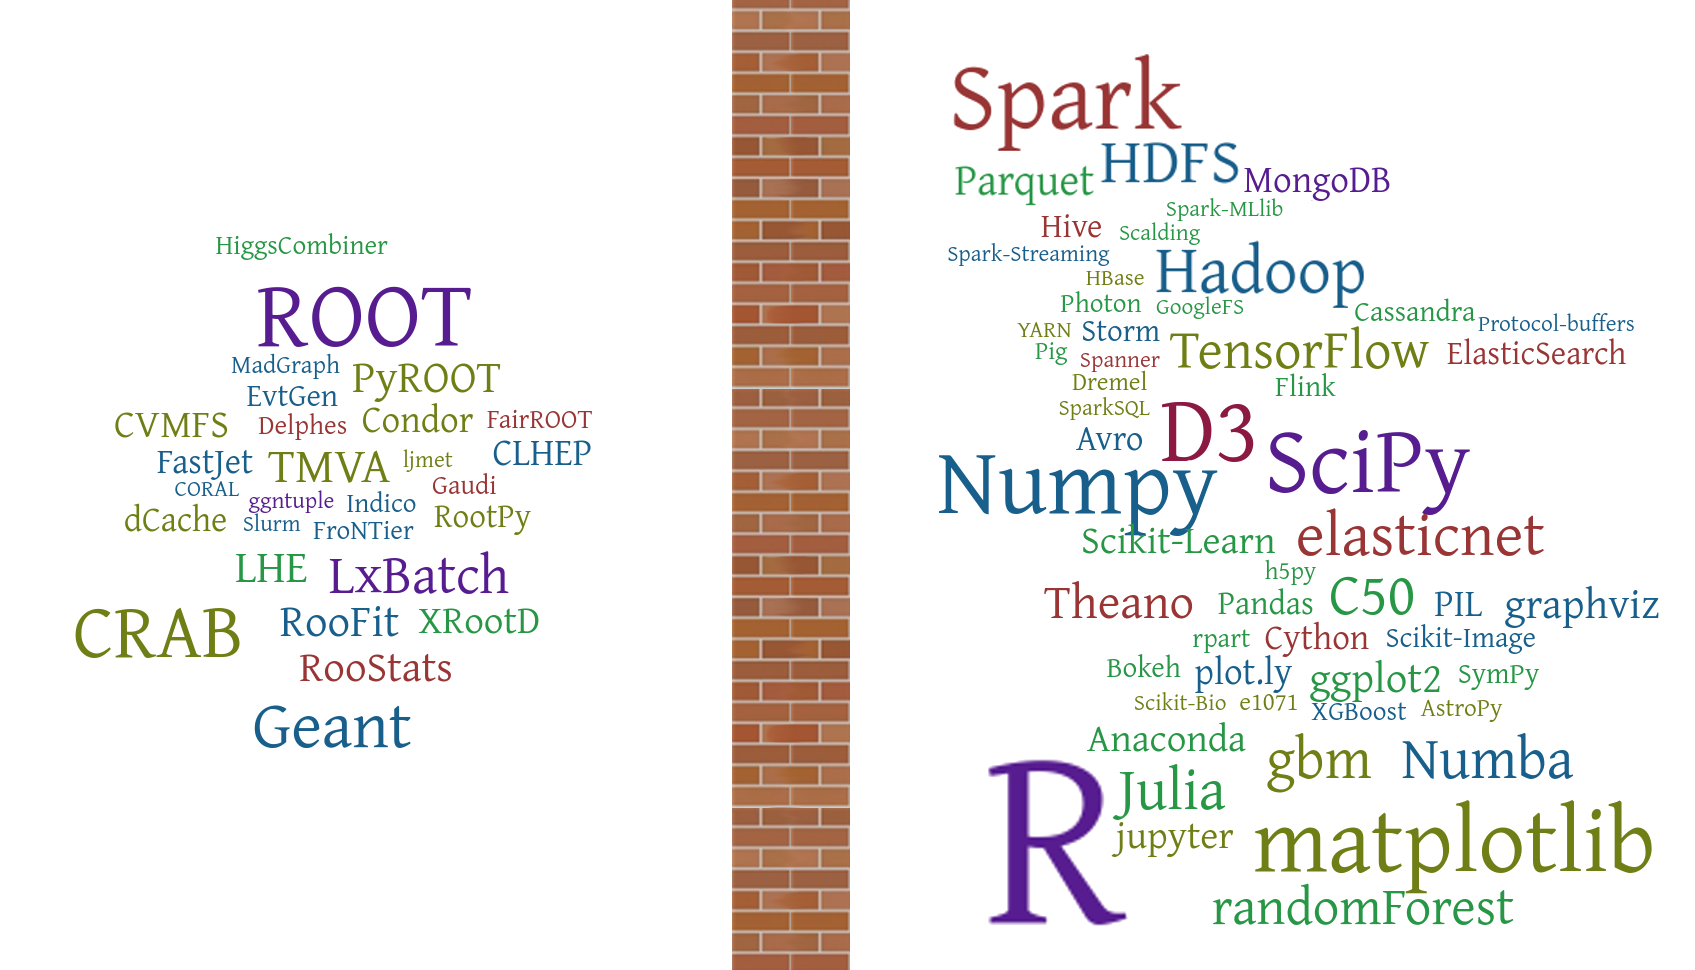
\includegraphics[width=\linewidth]{separation-2.png}
\end{frame}

\begin{frame}{Much of the Big Data software is developed for use in Python}
\vspace{0.5 cm}
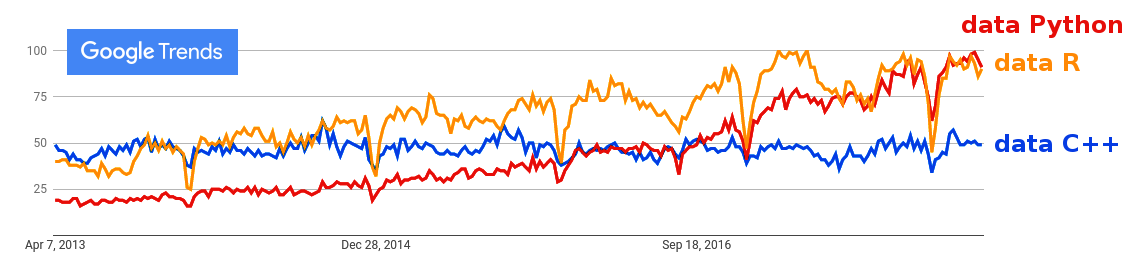
\includegraphics[width=\linewidth]{python-r-cpp-googletrends-data.png}

\vspace{1 cm}
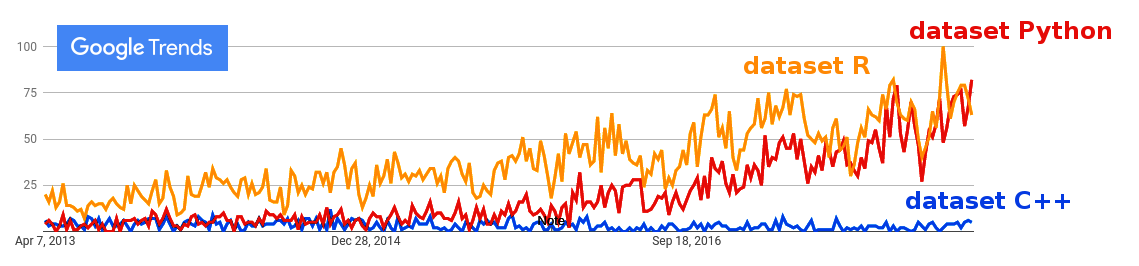
\includegraphics[width=\linewidth]{python-r-cpp-googletrends-dataset.png}
\end{frame}

\begin{frame}{Much of the Big Data software is developed for use in Python}
\vspace{0.5 cm}
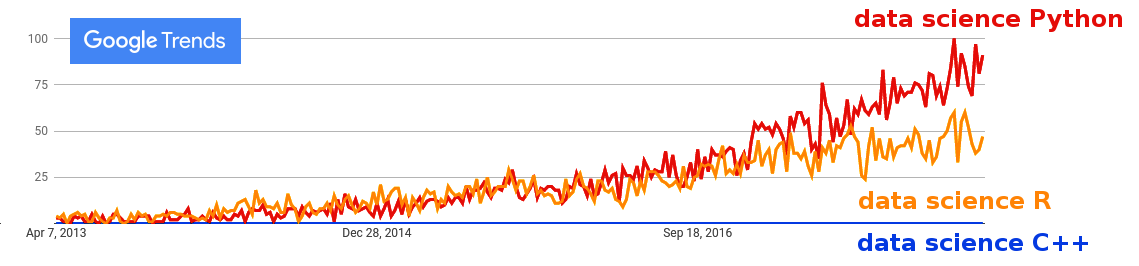
\includegraphics[width=\linewidth]{python-r-cpp-googletrends-datascience.png}

\vspace{1 cm}
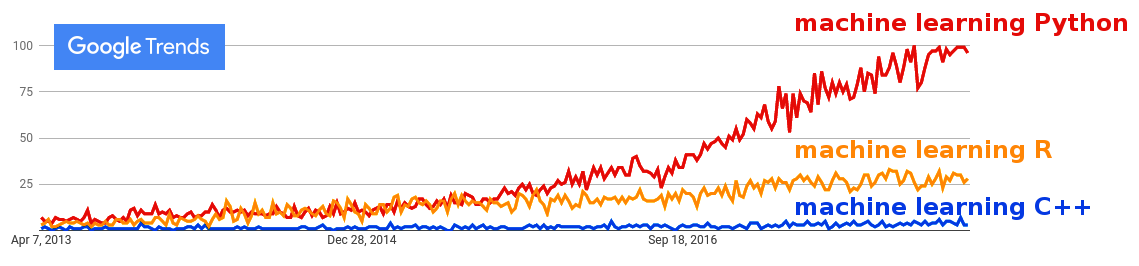
\includegraphics[width=\linewidth]{python-r-cpp-googletrends-machinelearning.png}
\end{frame}

\begin{frame}{The ``scientific Python ecosystem''}
\vspace{0.35 cm}
\textcolor{darkblue}{The word ``ecosystem'' is deliberately vague: no clear boundaries, but a few key components and many projects that share conventions.}

\begin{columns}
\column{1.1\linewidth}
\only<1>{
\includegraphics[width=\linewidth]{software-ecosystem-1.pdf}}
\only<2>{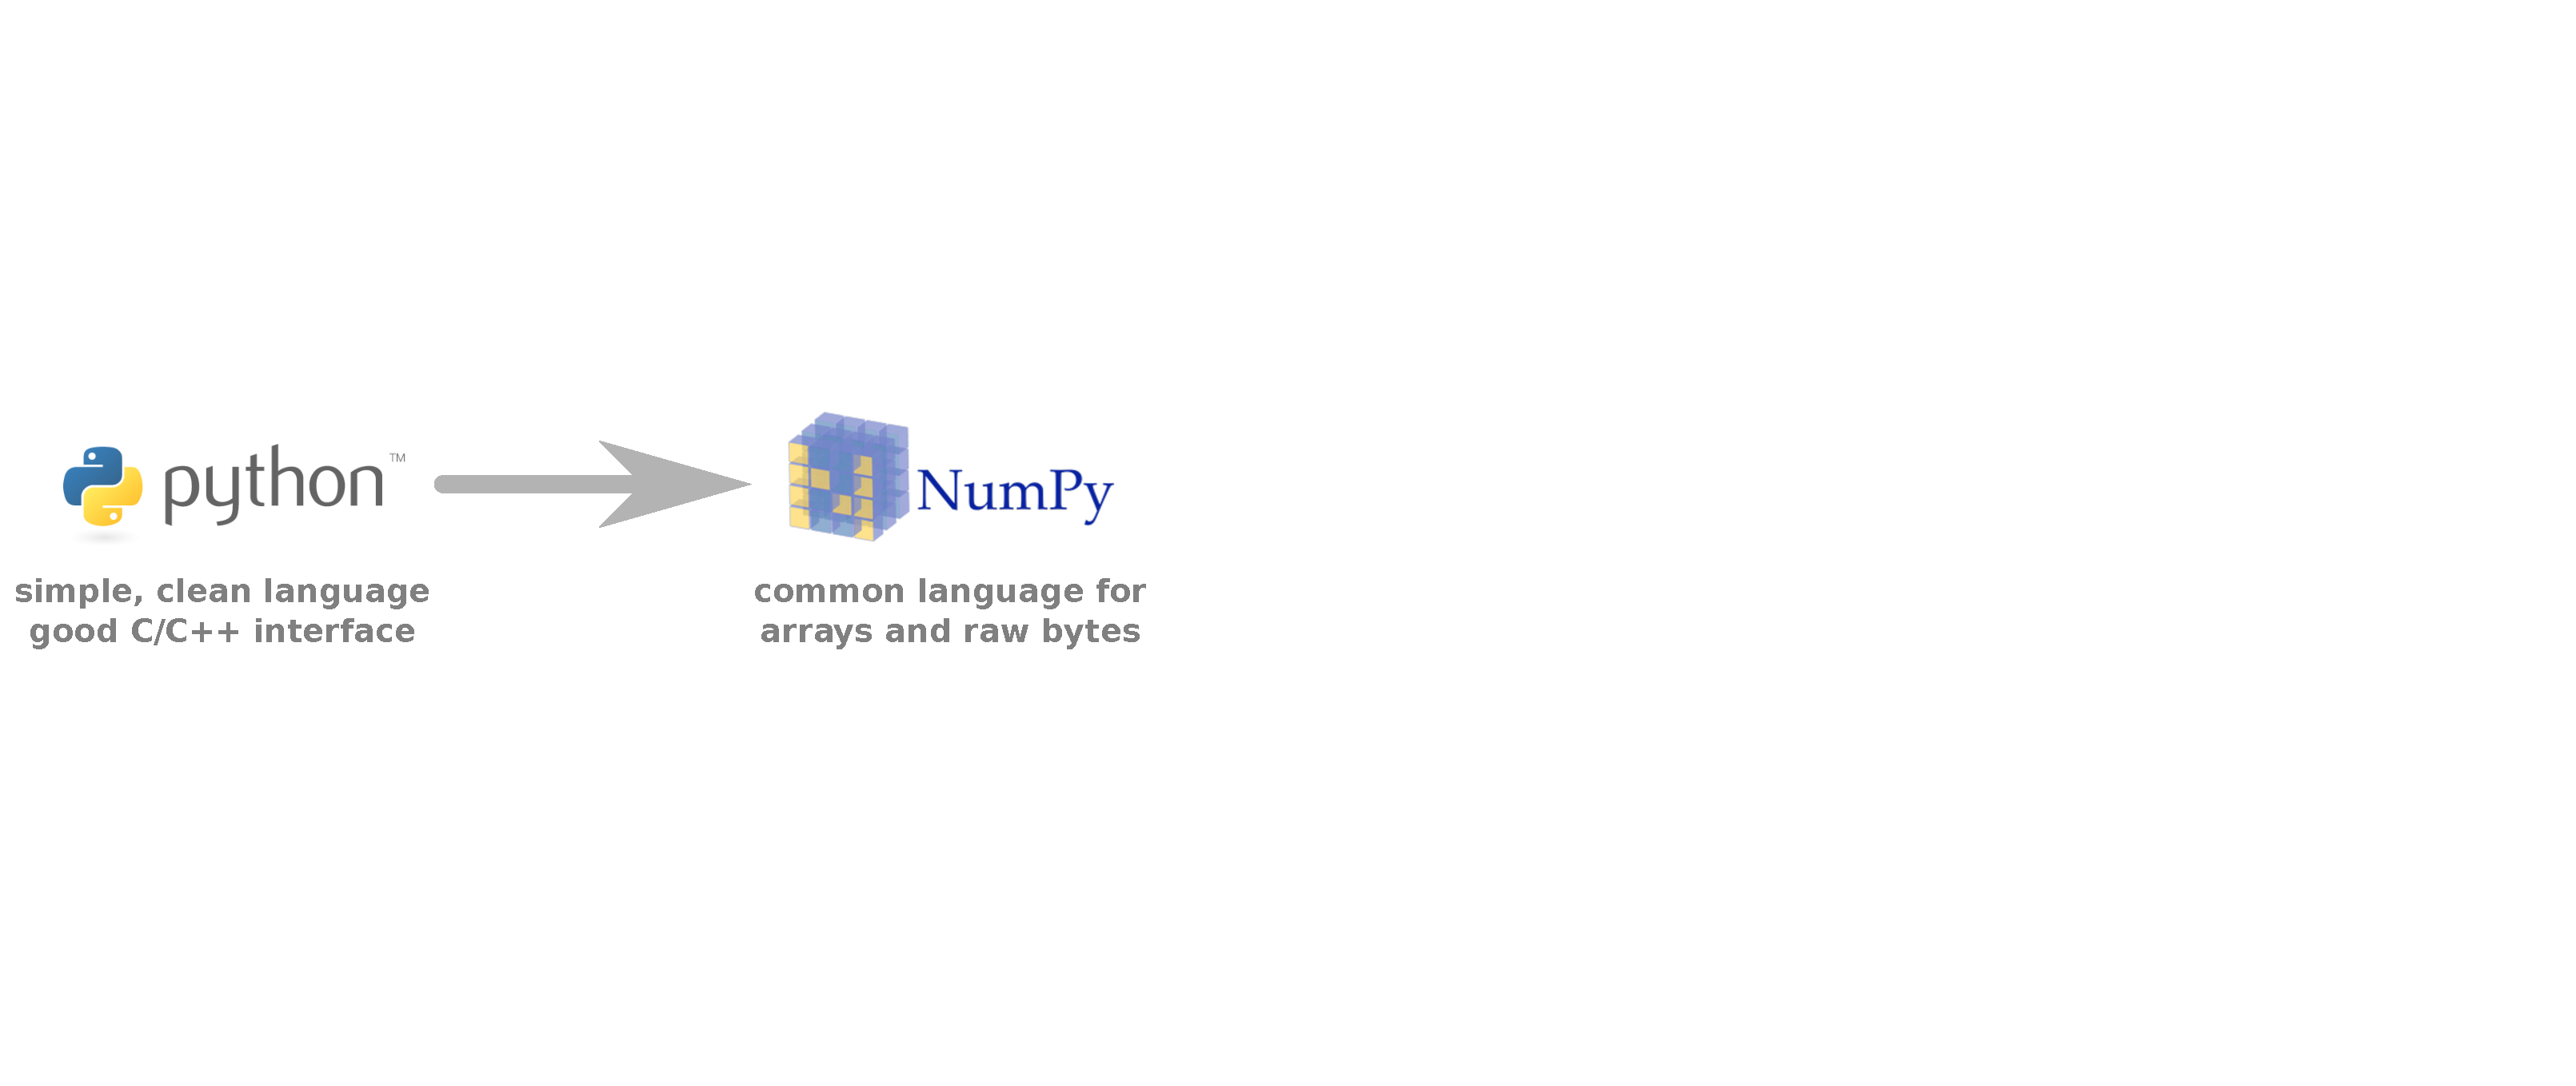
\includegraphics[width=\linewidth]{software-ecosystem-2.pdf}}
\only<3>{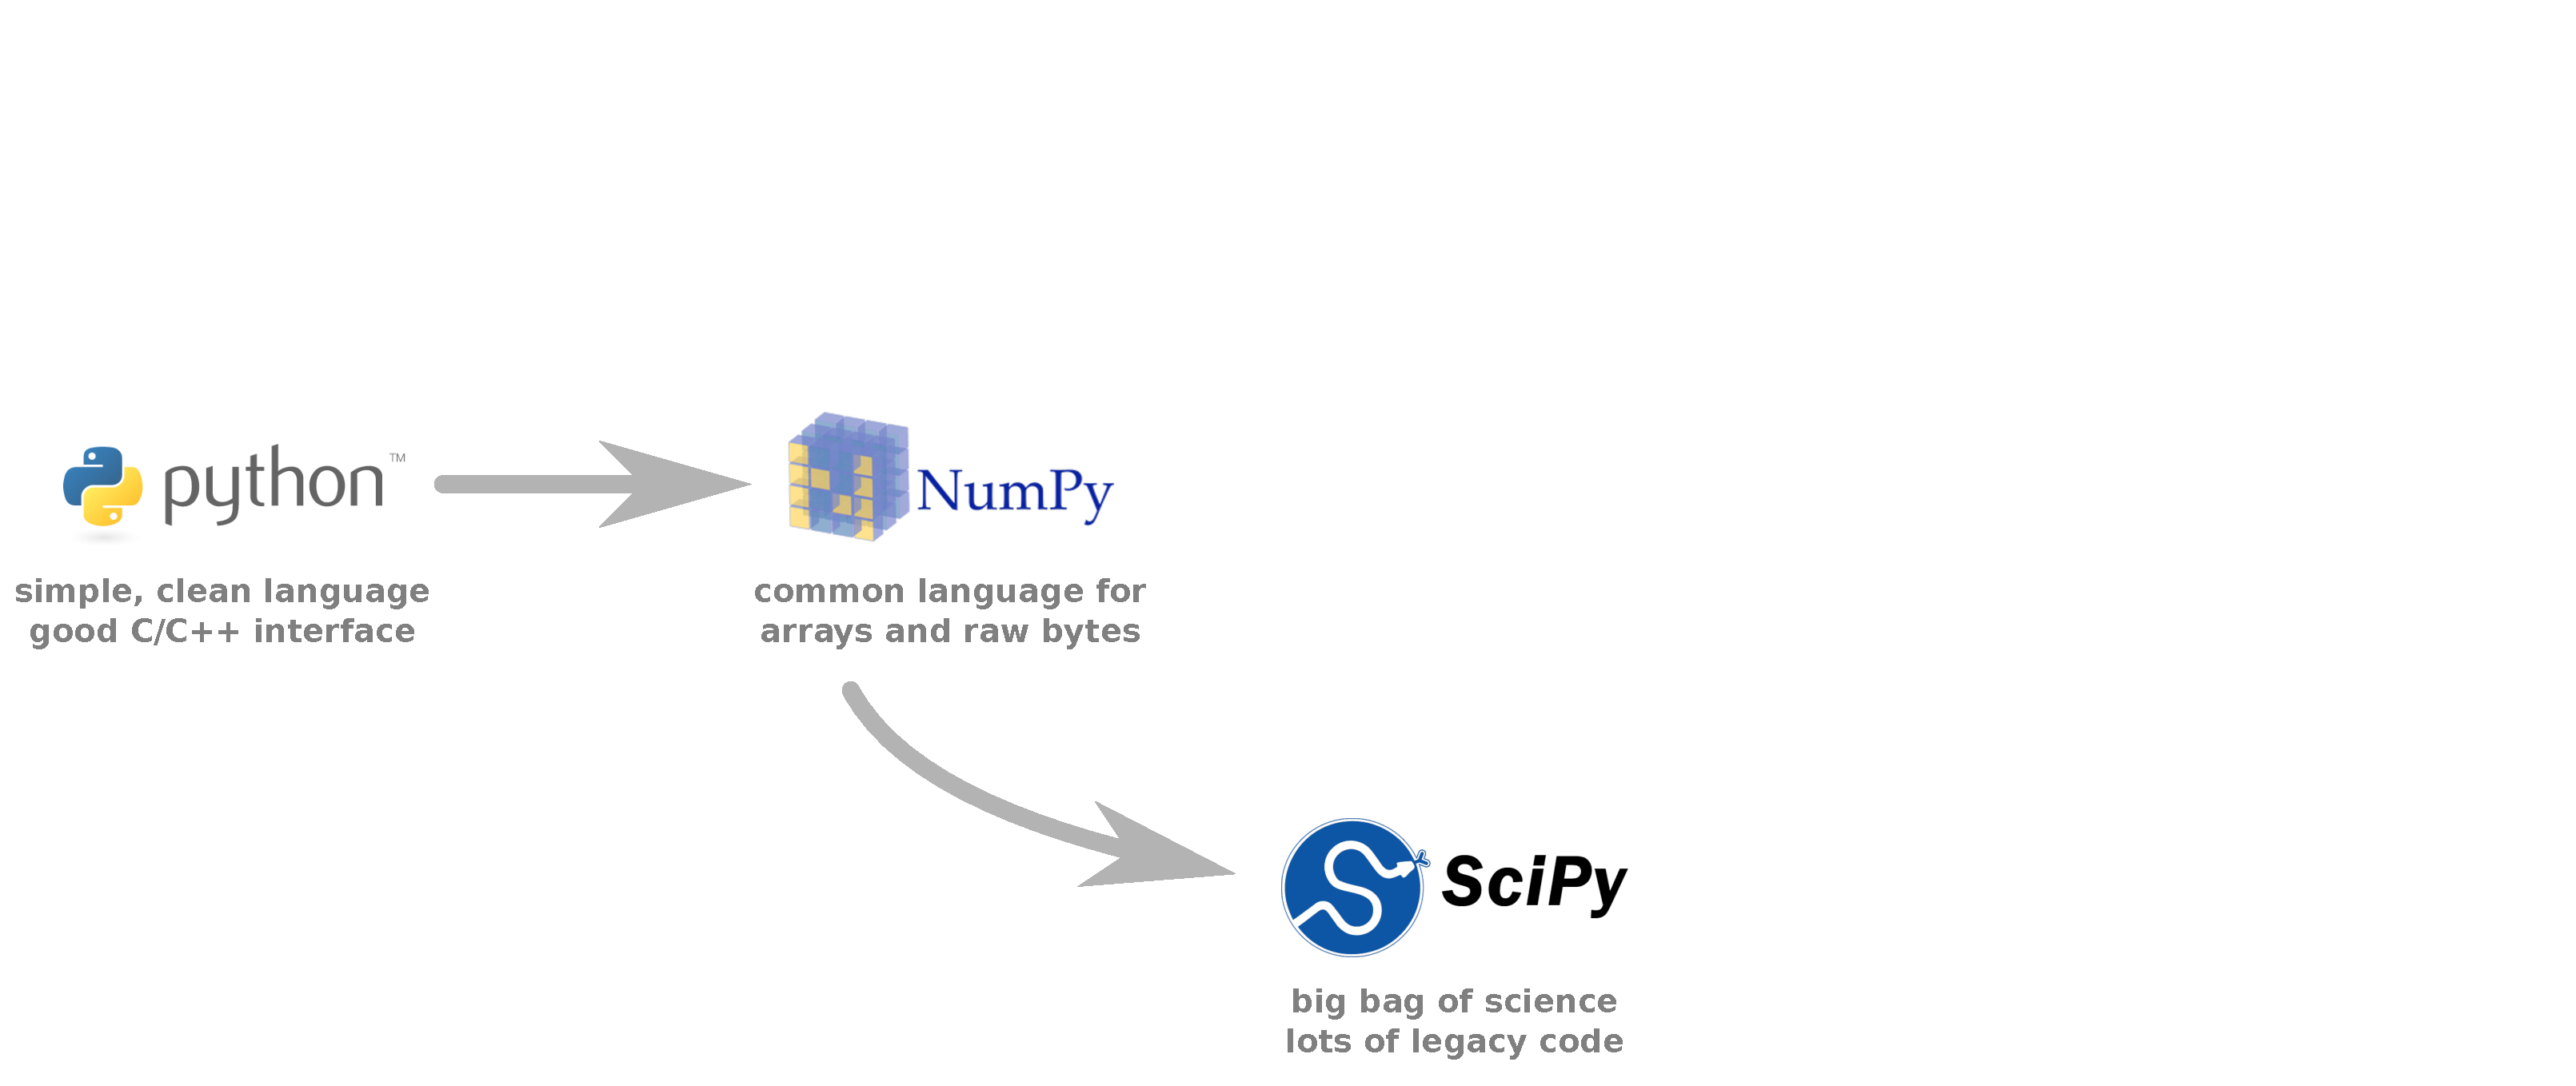
\includegraphics[width=\linewidth]{software-ecosystem-3.pdf}}
\only<4>{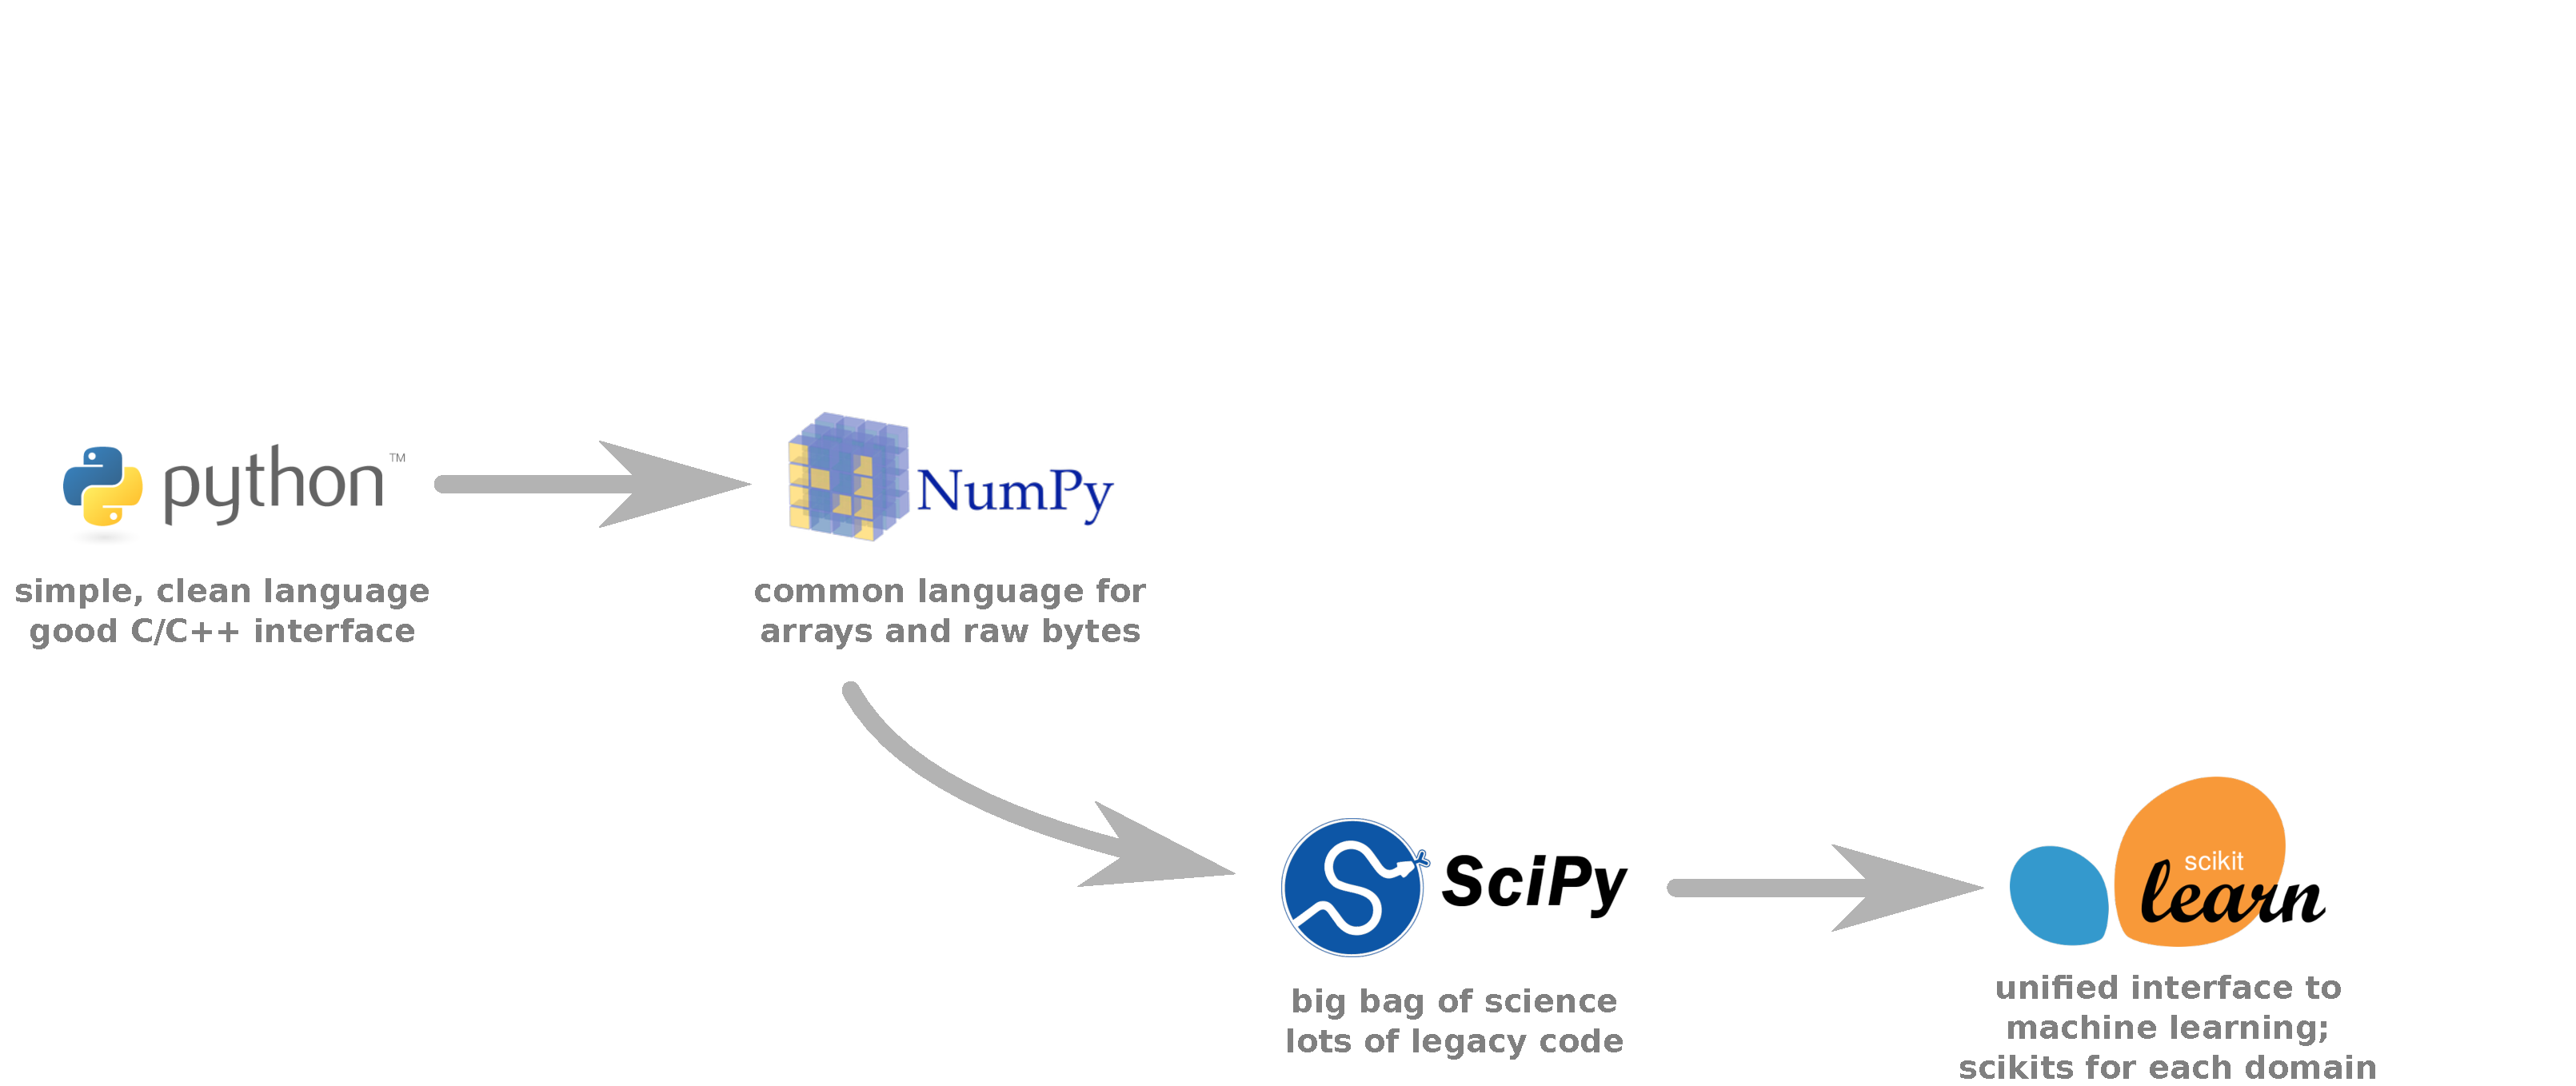
\includegraphics[width=\linewidth]{software-ecosystem-4.pdf}}
\only<5>{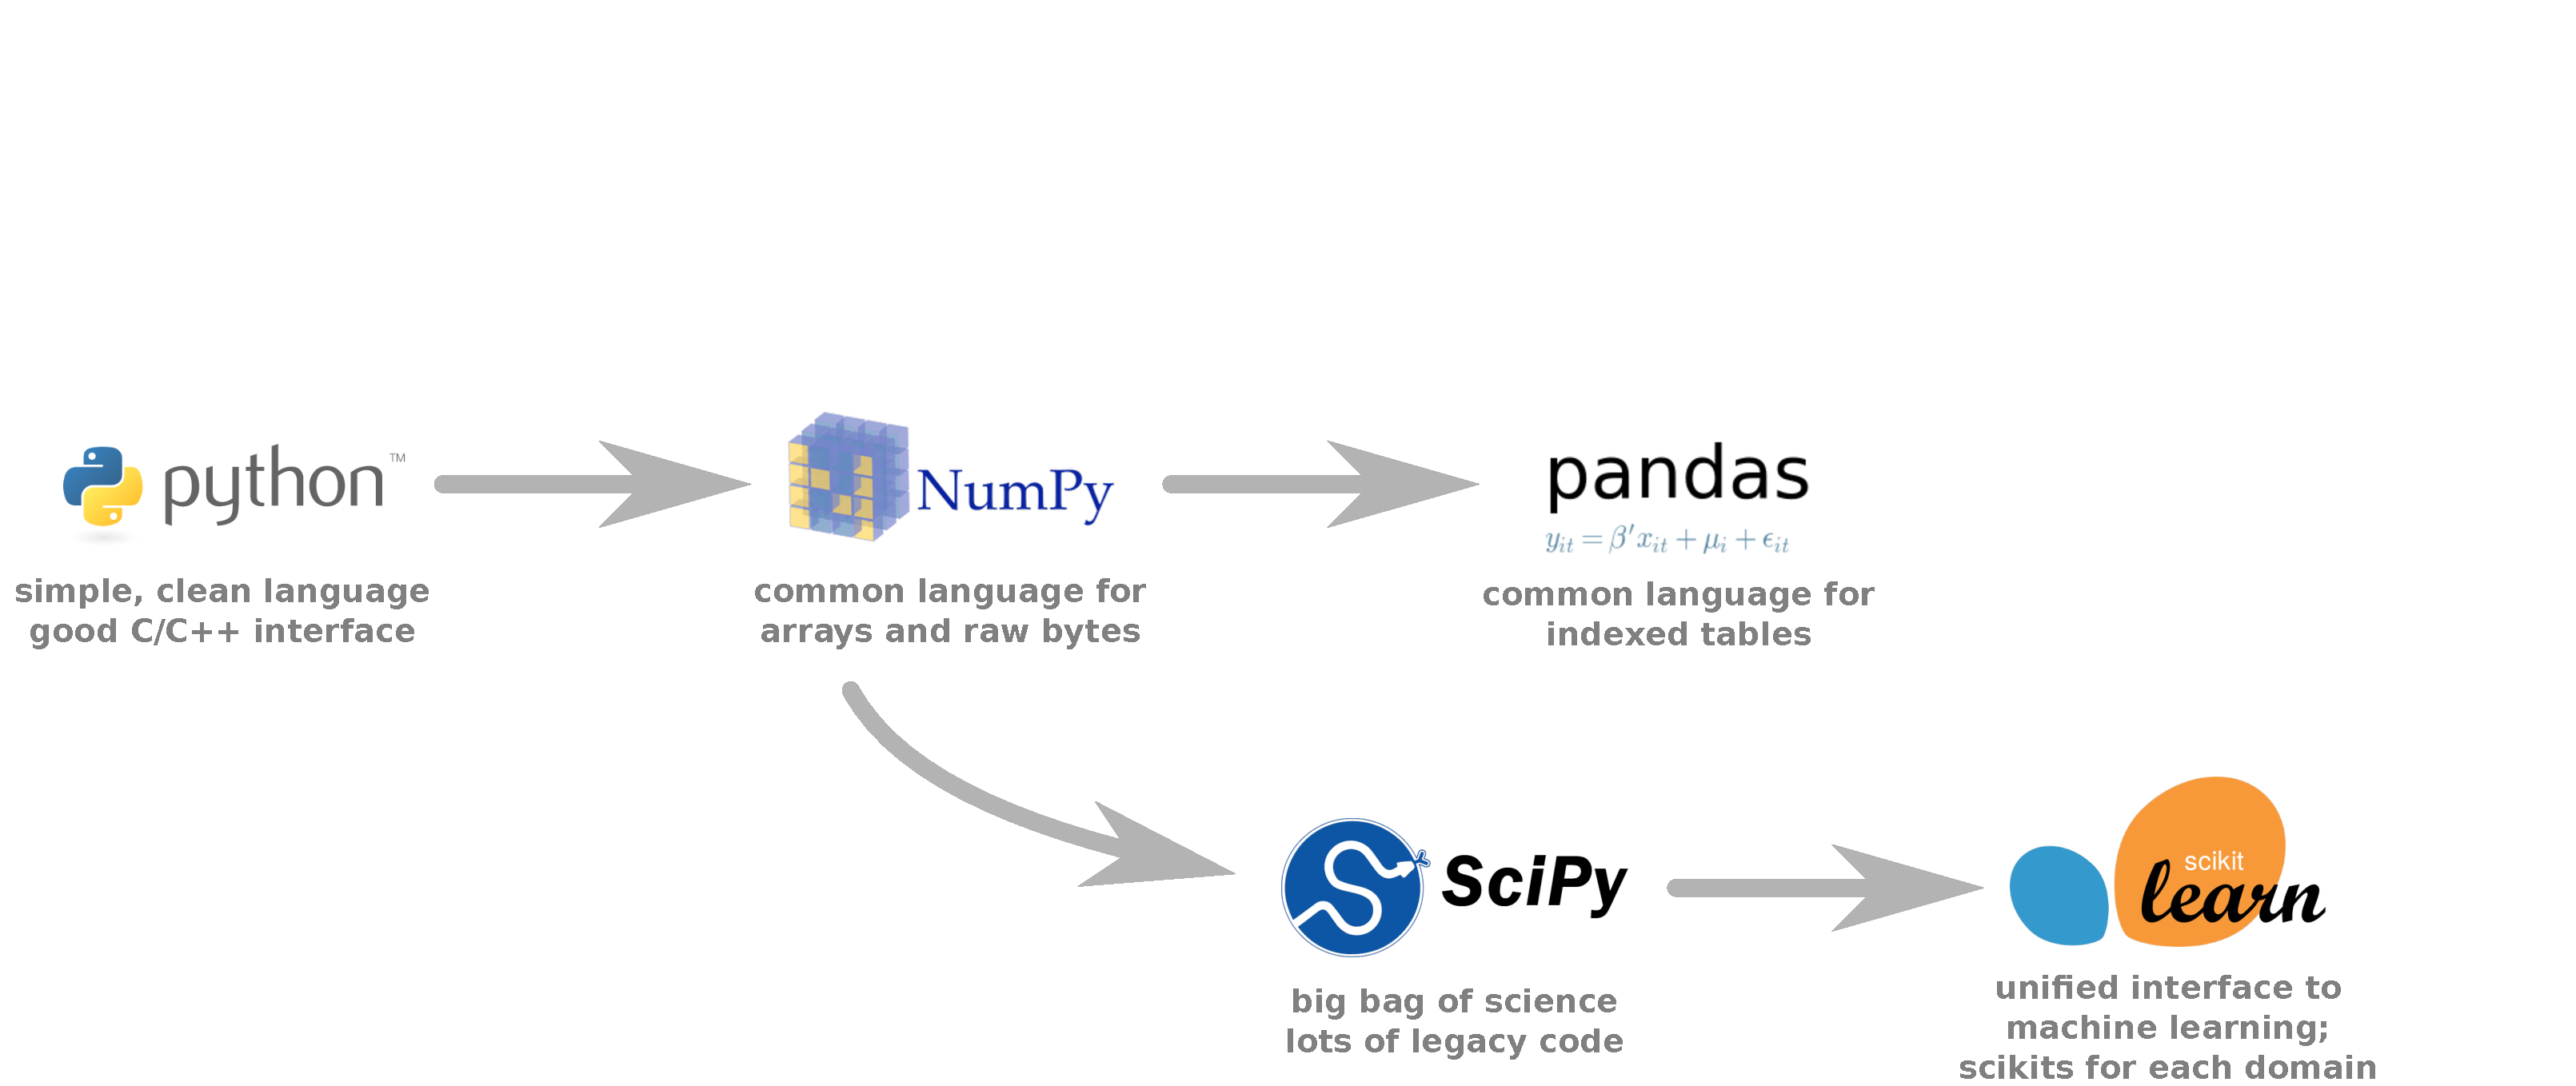
\includegraphics[width=\linewidth]{software-ecosystem-5.pdf}}
\only<6>{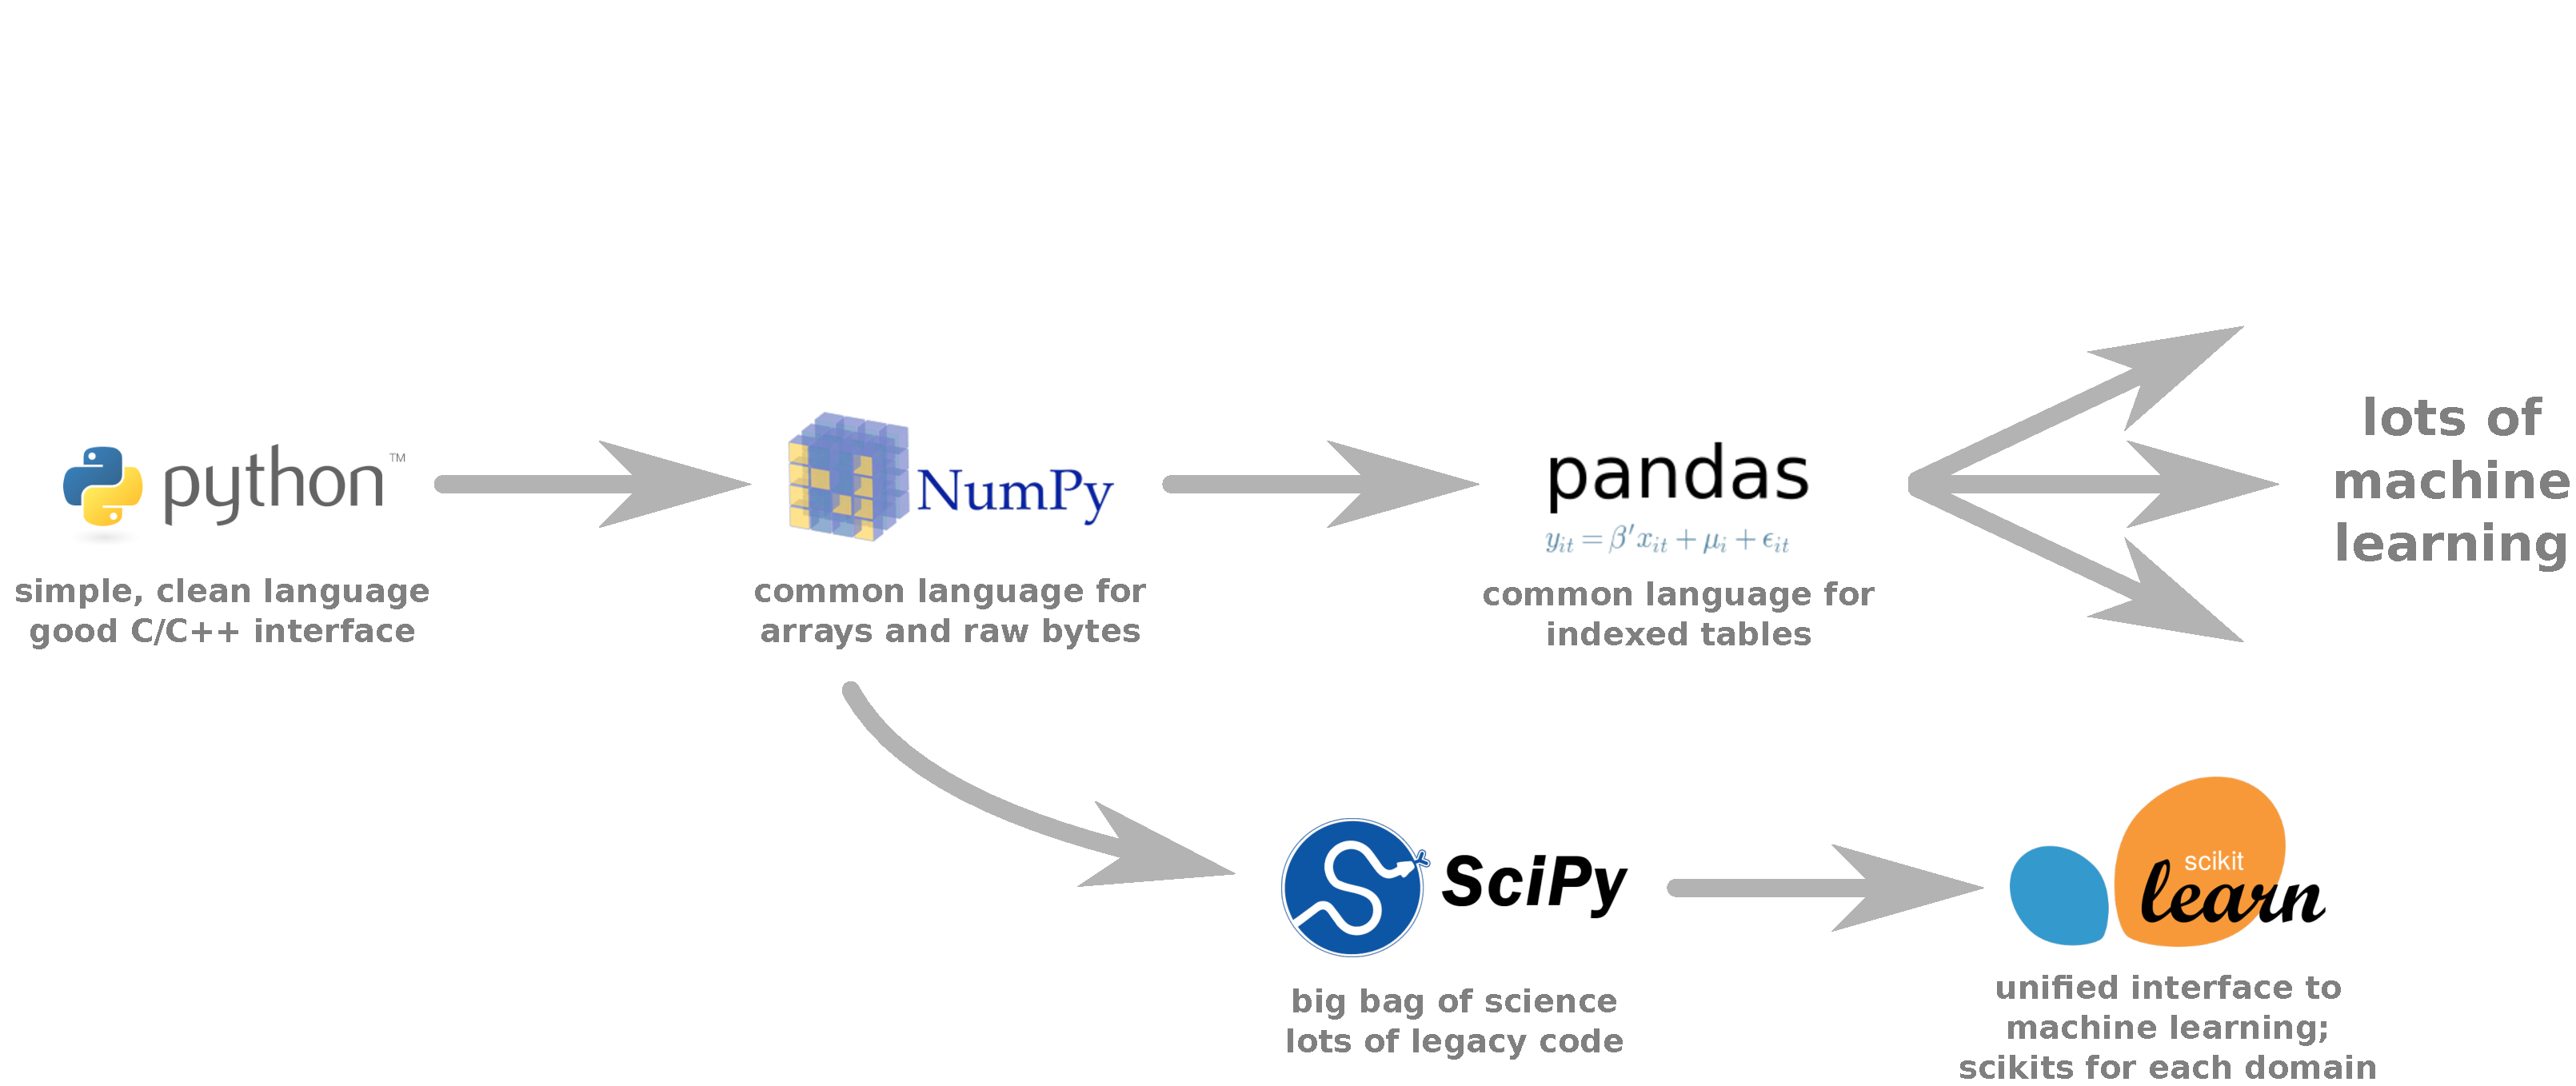
\includegraphics[width=\linewidth]{software-ecosystem-6.pdf}}
\only<7>{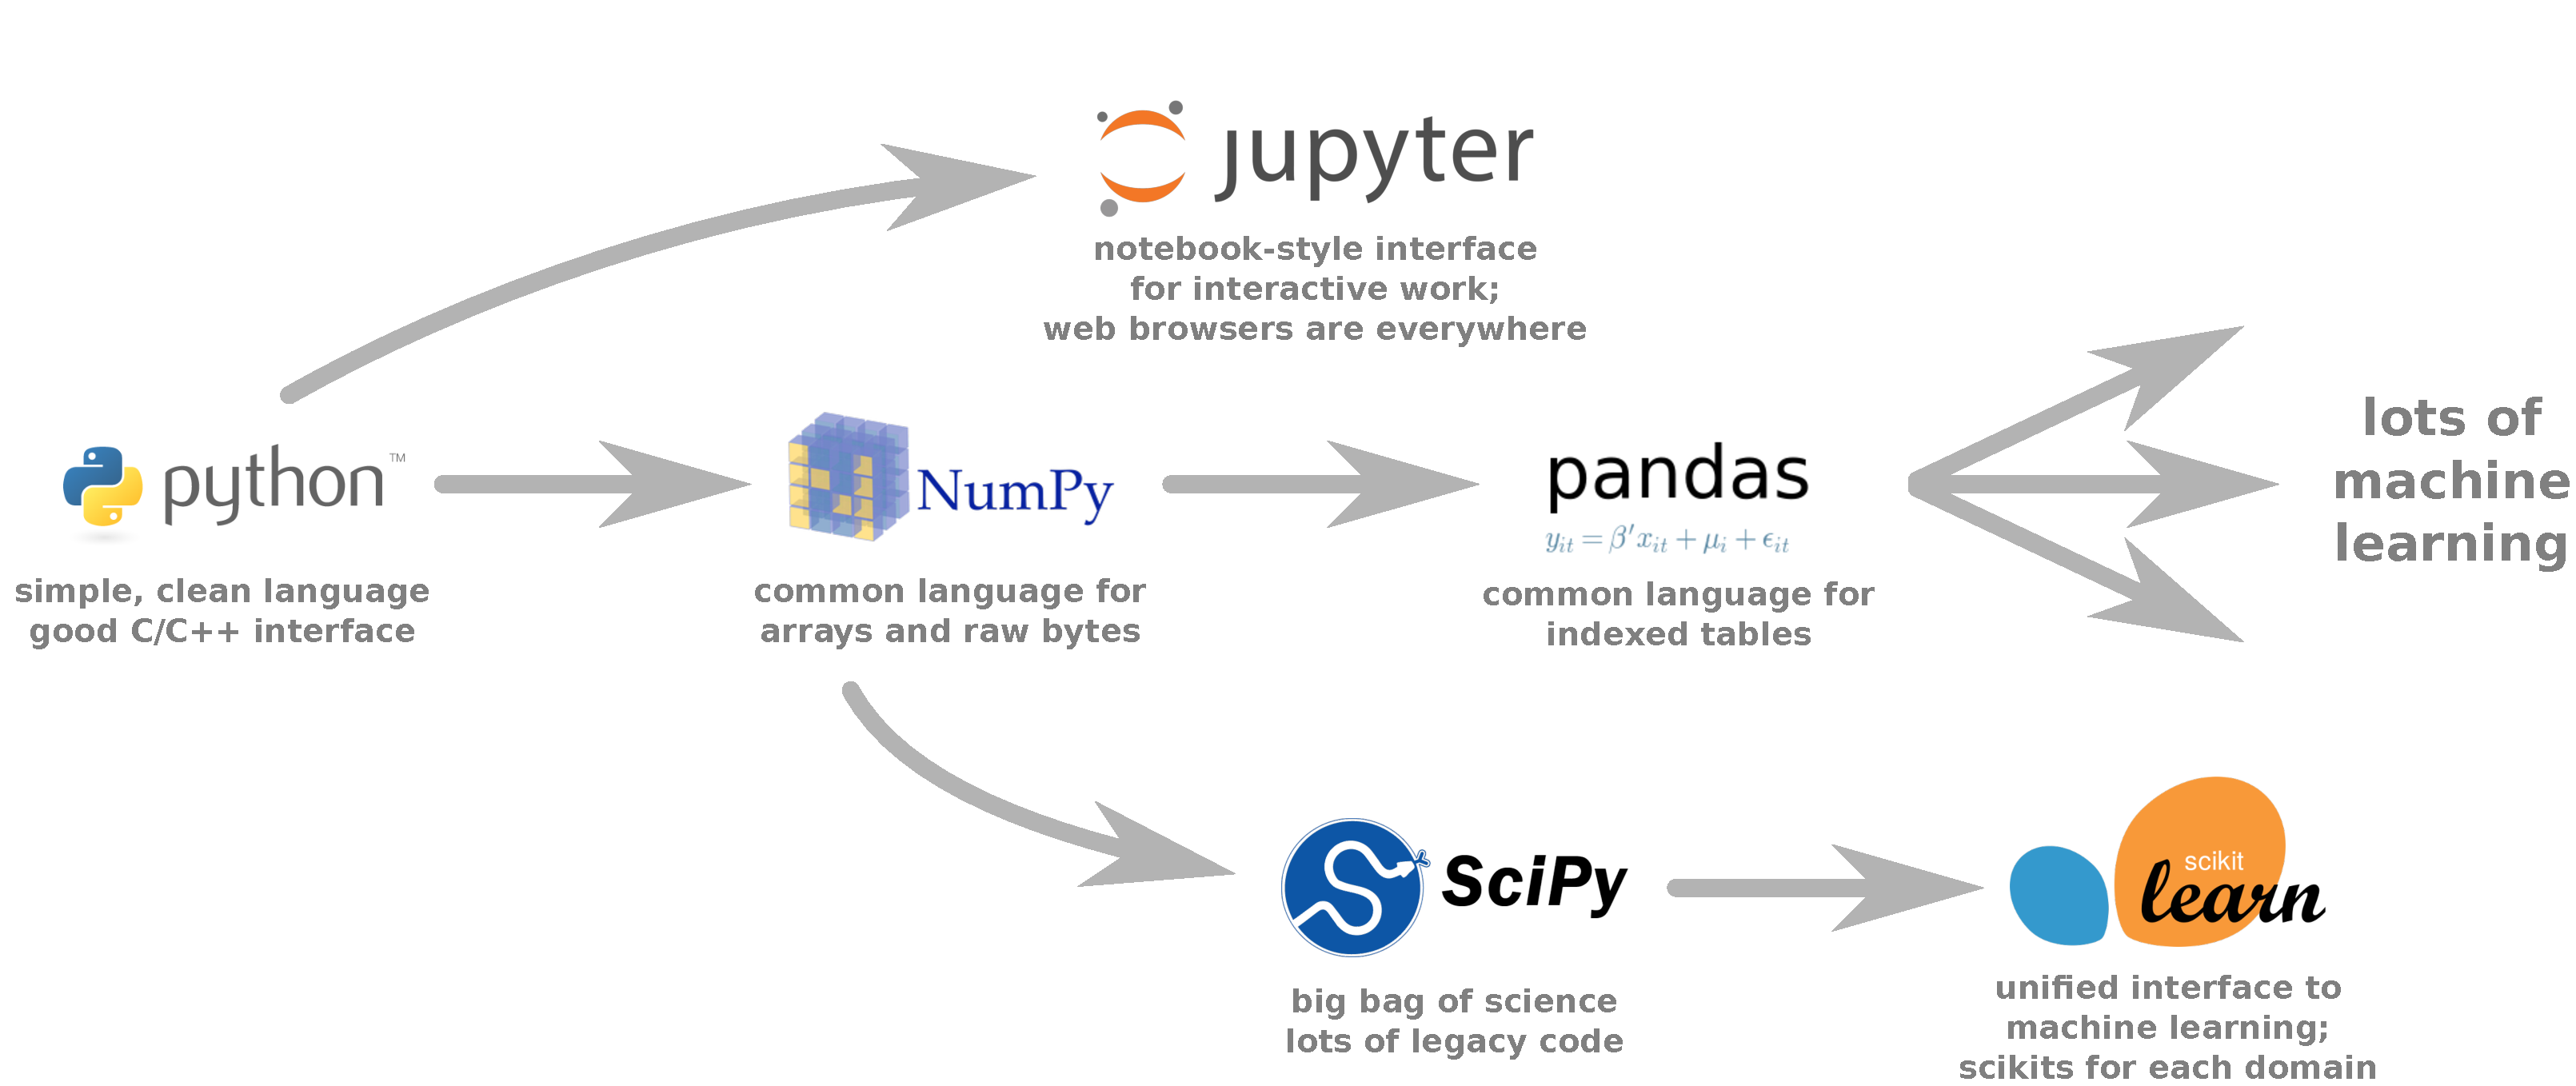
\includegraphics[width=\linewidth]{software-ecosystem-7.pdf}}
\only<8>{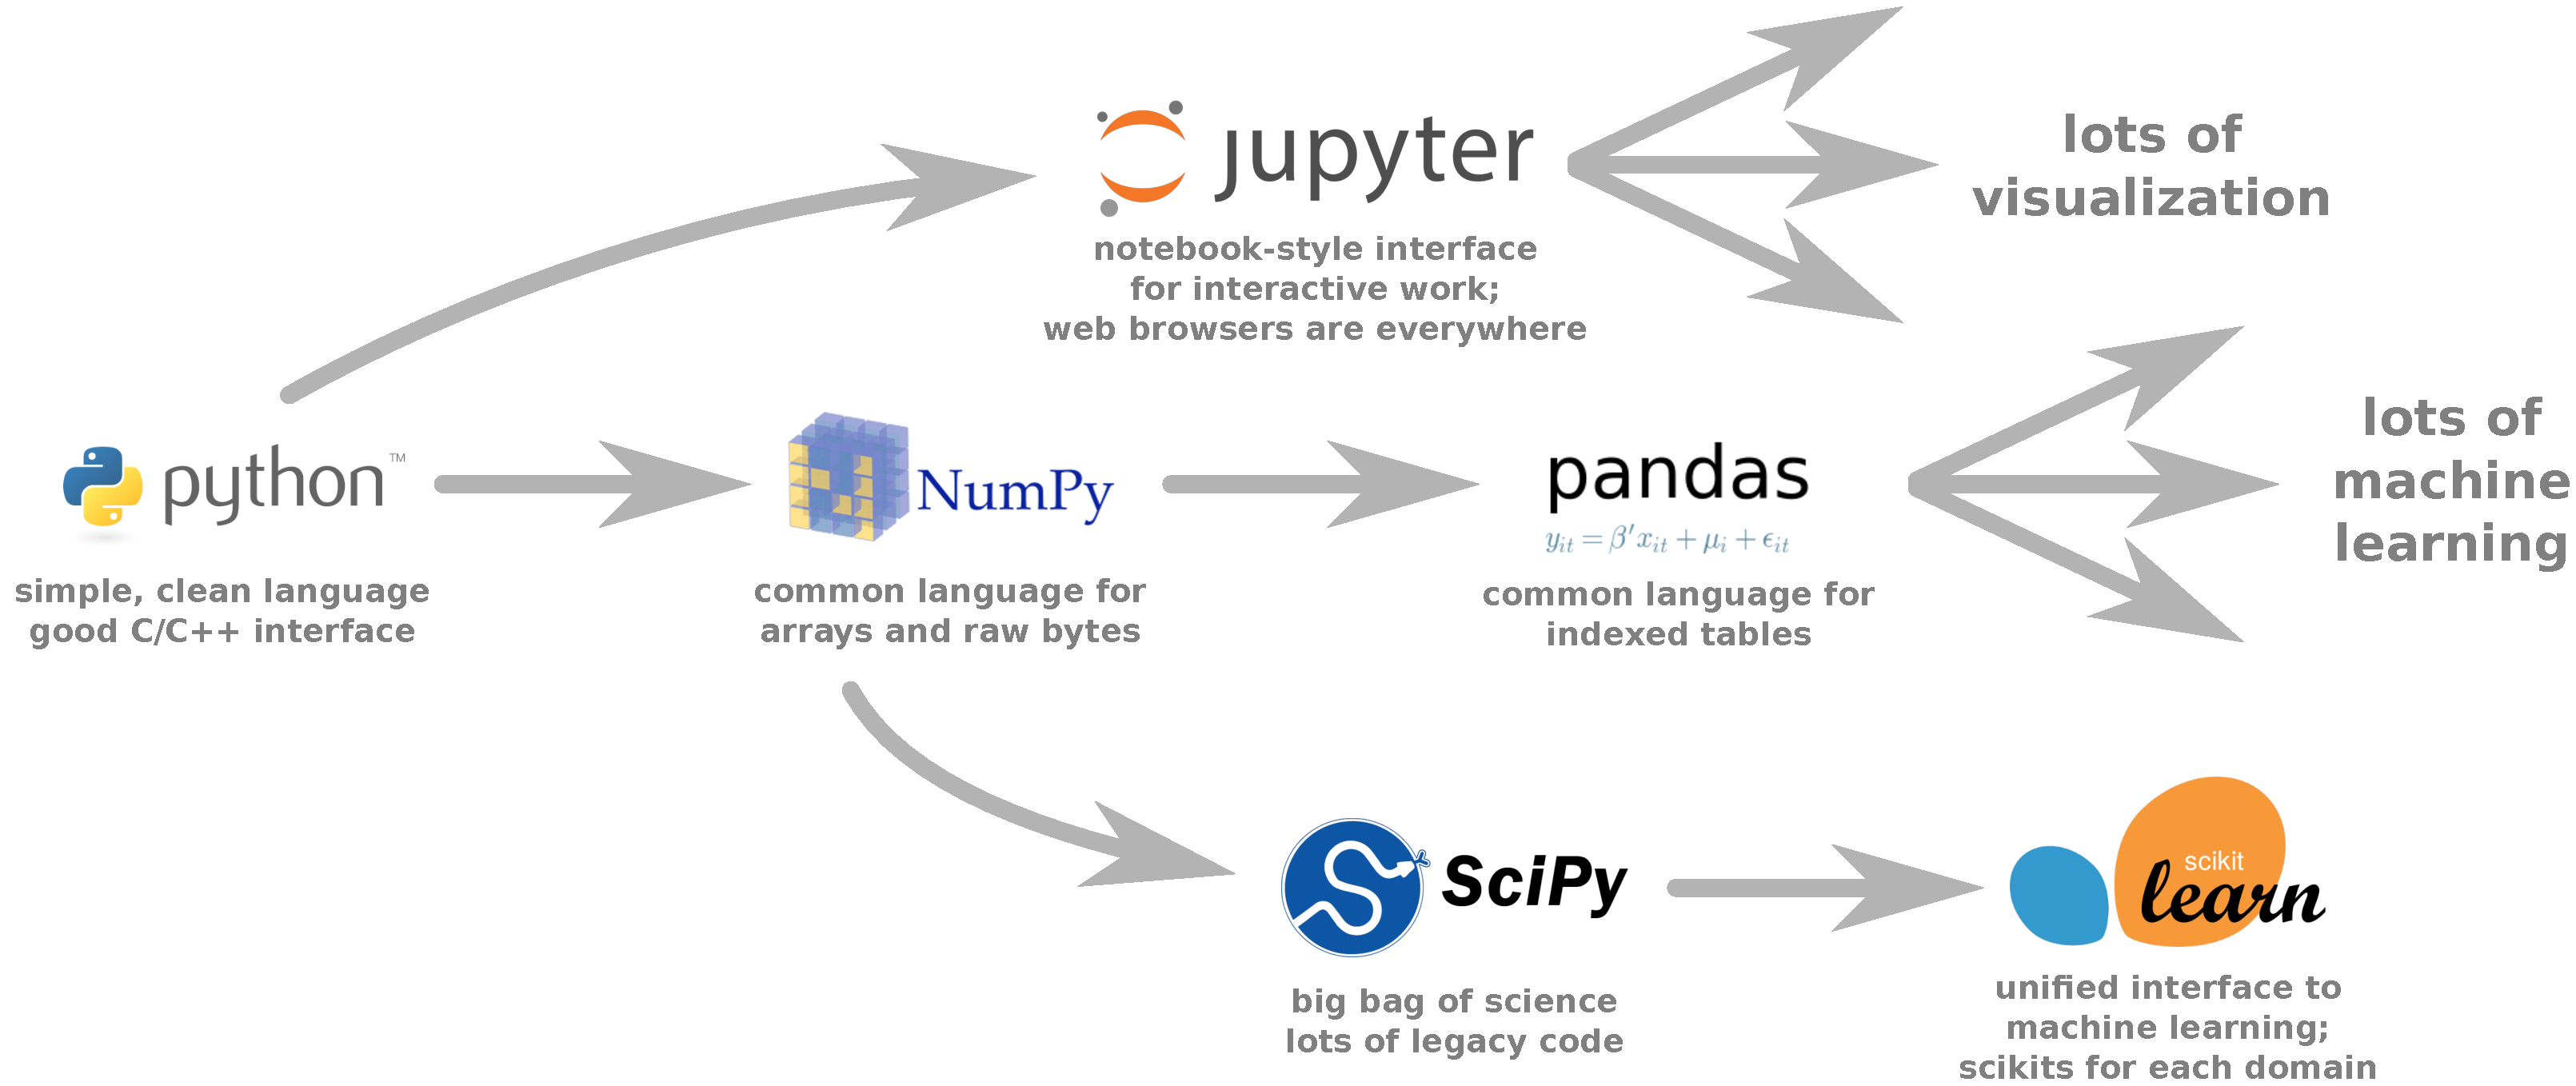
\includegraphics[width=\linewidth]{software-ecosystem-8.pdf}}
\end{columns}
\end{frame}

\begin{frame}{}
\begin{center}
\LARGE \textcolor{darkblue}{Key components of the ecosystem}
\end{center}
\end{frame}

\begin{frame}[fragile]{Python}
\vspace{0.5 cm}
\hfill 
\includegraphics[height=1 cm]{python-logo.png}

\vspace{-1 cm}
\begin{itemize}\setlength{\itemsep}{0.25 cm}
\item Convenient microsyntax, ``like executable pseudocode.''

Just for fun, try:

\small
\begin{minted}{python}
>>> import antigravity
\end{minted}
\normalsize

\item<2-> Abstraction and dynamism conspire to make programs written in Python slow.

\item<3-> However, CPython (the most popular implementation) has good bindings to C/C++. Scientific libraries are often written as a compiled number-crunching core with Pythonic interfaces.

\item<4-> The work of a data analyst is to drive the fast kernels from slow Python, or to glue interfaces to interfaces.
\end{itemize}

\vspace{0.25 cm}
\begin{uncoverenv}<5->
\small
\textcolor{darkblue}{Questions (show of hands):}
\vspace{-0.2 cm}
\begin{enumerate}\setlength{\itemsep}{-0.1 cm}
\item How many people have used Python a lot?
\item A little?
\item Not at all?
\end{enumerate}
\end{uncoverenv}
\end{frame}

\begin{frame}{Numpy}
\vspace{0.5 cm}
\hfill 
\includegraphics[height=1.3 cm]{numpy-logo.png}

\vspace{-1.3 cm}
Python wasn't practical for science before Numpy.

(Numarray vs.\ Numeric split community $\to$ Numpy in 2006.)

\vspace{0.35 cm}
\begin{uncoverenv}<2->
\textcolor{darkblue}{Promotes ``vectorized'' calculations.}

\begin{center}
\begin{minipage}{0.85\linewidth}
Taco chef can make 8~tacos of the same type in the same time as 1.5~tacos.

\vspace{0.2 cm}
If customers order different types of tacos \`a la carte, the chef will take a lot longer than if orders of the same type are batched.
\end{minipage}
\end{center}
\end{uncoverenv}

\vspace{0.15 cm}
\begin{columns}[t]
\column{0.46\linewidth}
\begin{uncoverenv}<3->
\textcolor{darkblue}{In Numpy, $\sqrt{x^2 + y^2}$ is}
\begin{enumerate}
\item square all the $x$ (for all events)
\item square all the $y$ (for all events)
\item add them (for all events)
\item take the square root (for all events)
\end{enumerate}
\end{uncoverenv}

\column{0.46\linewidth}
\uncover<4->{Dealing with a single Python instruction takes a lot longer than squaring or adding hundreds of numbers, so ``batching math'' saves time.}

\vspace{0.15 cm}
\uncover<5->{\textcolor{darkblue}{\underline{Similar} to hardware vectorization:} optimizing for GPUs and modern CPUs.}
\end{columns}
\end{frame}

\begin{frame}{Numpy}
\vspace{0.5 cm}
Algorithms that transform one input into one output are easy to vectorize.

\vspace{0.15 cm}
\mbox{\hspace{0.5 cm}}$\longrightarrow$ flat ntuples (tables of numbers) are good for Numpy.

\vspace{0.25 cm}
\begin{uncoverenv}<2->
Algorithms with nested for loops are harder to think about.

\vspace{0.15 cm}
\mbox{\hspace{0.5 cm}}$\longrightarrow$ e.g.\ TTrees containing {\tt\small std::vectors}
\end{uncoverenv}

\vspace{0.25 cm}
\begin{center}
\begin{minipage}{0.85\linewidth}
\uncover<3->{\textcolor{darkblue}{OAMap (object-array mapping)} is a tool I've developed to bridge the two worlds: to let you write standard for-loop/object-like code and execute it without performance loss on arrays.}
\end{minipage}
\end{center}

\vspace{0.25 cm}
\begin{uncoverenv}<4->
\small
\textcolor{darkblue}{Questions (show of hands):}
\vspace{-0.2 cm}
\begin{enumerate}\setlength{\itemsep}{-0.1 cm}
\item How many people have performed vectorized calculations in Numpy?
\item How many have used Numpy at all?
\item How many haven't?
\end{enumerate}
\end{uncoverenv}
\end{frame}

\begin{frame}{SciPy libraries}
\vspace{0.35 cm}
\hfill 
\includegraphics[height=1 cm]{scipy-logo.png}

\vspace{-1 cm}
\begin{columns}[b]
\column{0.5\linewidth}
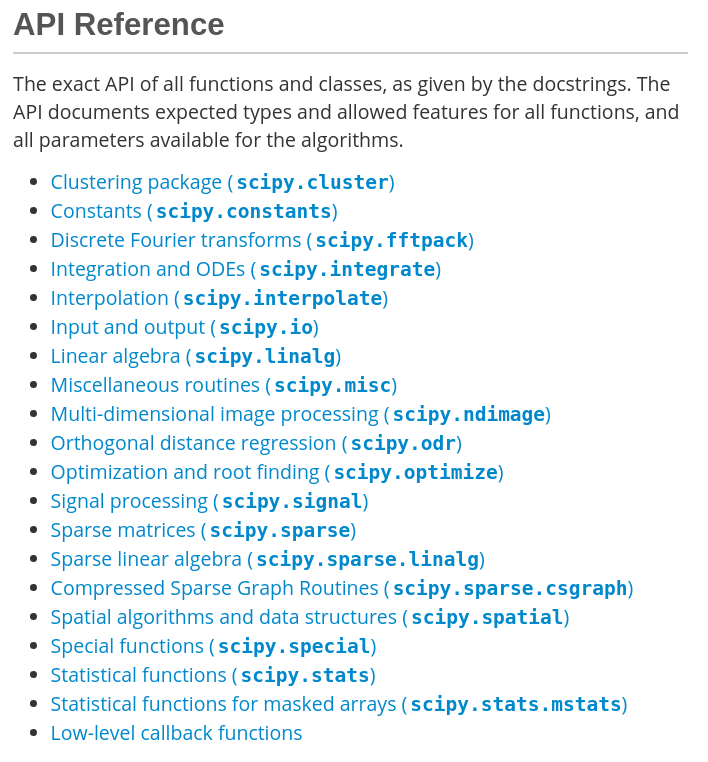
\includegraphics[width=\linewidth]{scipy-docs.png}

\column{0.5\linewidth}
SciPy is like Python's ROOT: all the classic algorithms with references to the literature.

\vspace{0.2 cm}
\uncover<2->{Many of these are the original Fortran implementations, wrapped in Python.}

\vspace{0.2 cm}
\uncover<3->{Unlike Numpy and Pandas, SciPy isn't something you need fluency in--- it's a bag of functions you dig into on occasion.}

\vspace{0.5 cm}
\begin{uncoverenv}<4->
\small
\textcolor{darkblue}{Questions (show of hands):}
\vspace{-0.2 cm}
\begin{enumerate}\setlength{\itemsep}{-0.1 cm}
\item How many people have used at least one function from SciPy?
\item How many haven't?
\end{enumerate}
\end{uncoverenv}
\vspace{0.05 cm}
\end{columns}
\end{frame}



%% \begin{frame}{Pandas data frames}
%% \vspace{0.35 cm}
%% \hfill 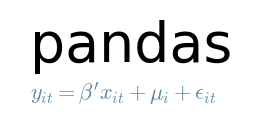
\includegraphics[height=1.3 cm]{pandas-logo.png}

%% \vspace{-1.3 cm}
%% Numpy provides in-memory data tables with slick indexing.

%% \vspace{0.05 cm}
%% \uncover<2->{Pandas provides in-memory data tables with slick indexing.}

%% \vspace{0.05 cm}
%% \uncover<3->{Pandas is considered an enabling technology for data science.}

%% \vspace{0.35 cm}
%% \uncover<4->{\textcolor{darkblue}{What's the big deal?}}

%% \begin{itemize}\setlength{\itemsep}{0.1 cm}
%% \item<5-> The rows of Pandas data frames are indexed: each row {\it means} something.

%% \vspace{0.1 cm}
%% \uncover<6->{For example, adding two data frames with different sets of keys matches the overlapping sets of keys and unions the others: more like a {\tt\small dict} than a {\tt\small list}.}

%% \vspace{0.1 cm}
%% \uncover<7->{$\longrightarrow$ Think ``systematics studies,'' not ``bag of events!''}

%% \item<8-> Includes built-in plotting and statistics.

%% \item<9-> Common target for user-oriented statistical packages, especially machine learning.
%% \end{itemize}

%% \vspace{0.35 cm}
%% \begin{uncoverenv}<10->
%% \small
%% \textcolor{darkblue}{Questions (show of hands):}
%% \vspace{-0.2 cm}
%% \begin{enumerate}\setlength{\itemsep}{-0.1 cm}
%% \item How many people have used Pandas?
%% \item How many haven't?
%% \end{enumerate}
%% \end{uncoverenv}
%% \end{frame}


%% \begin{frame}{Jupyter notebooks}
%% \vspace{0.4 cm}
%% \hfill 
\includegraphics[height=0.8 cm]{jupyter-logo.png}

%% \vspace{-0.8 cm}
%% \underline{There are fundamentally four ways to use a computer:}

%% \vspace{0.15 cm}
%% \begin{enumerate}
%% \item<2-> \textcolor{darkblue}{Batch:} write a series of instructions (punchcards or script), \\ run the whole thing, interpret results, maybe do it again with corrections.
%% \item<3-> \textcolor{darkblue}{Prompt:} submit a command, see the results, think, submit another command.
%% \item<4-> \textcolor{darkblue}{Notebook:} interactivity of prompt, but overwriting mistaken commands to build up a reusable script. \textcolor{gray}{(Interleaving text and graphics is {\it optional.})}
%% \item<5-> \textcolor{darkblue}{Graphical:} point-and-click or touchscreen; easy but limited in scope.
%% \end{enumerate}

%% \vspace{0.25 cm}
%% \uncover<6->{Notebook-style interaction is \underline{\it incredibly useful for data analysis} because you must be able to quickly iterate through mistakes, but then also finalize a procedure.}

%% \vspace{0.25 cm}
%% \uncover<7->{If you haven't decided on a text editor yet, consider \href{https://mybinder.org/v2/gh/jupyterlab/jupyterlab-demo/master?urlpath=lab/tree/demo}{\textcolor{blue}{JupyterLab}}. \textcolor{gray}{\tiny (Personally, I'll die with Emacs.)}}

%% \vspace{0.35 cm}
%% \begin{uncoverenv}<8->
%% \small
%% \textcolor{darkblue}{Questions (show of hands):}
%% \vspace{-0.2 cm}
%% \begin{enumerate}\setlength{\itemsep}{-0.1 cm}
%% \item Is this your first time using Jupyter?
%% \item Do you plan on using it for normal work?
%% \end{enumerate}
%% \end{uncoverenv}
%% \end{frame}

%% \begin{frame}{JupyterLab is a realistically usable editor}
%% \vspace{0.35 cm}
%% 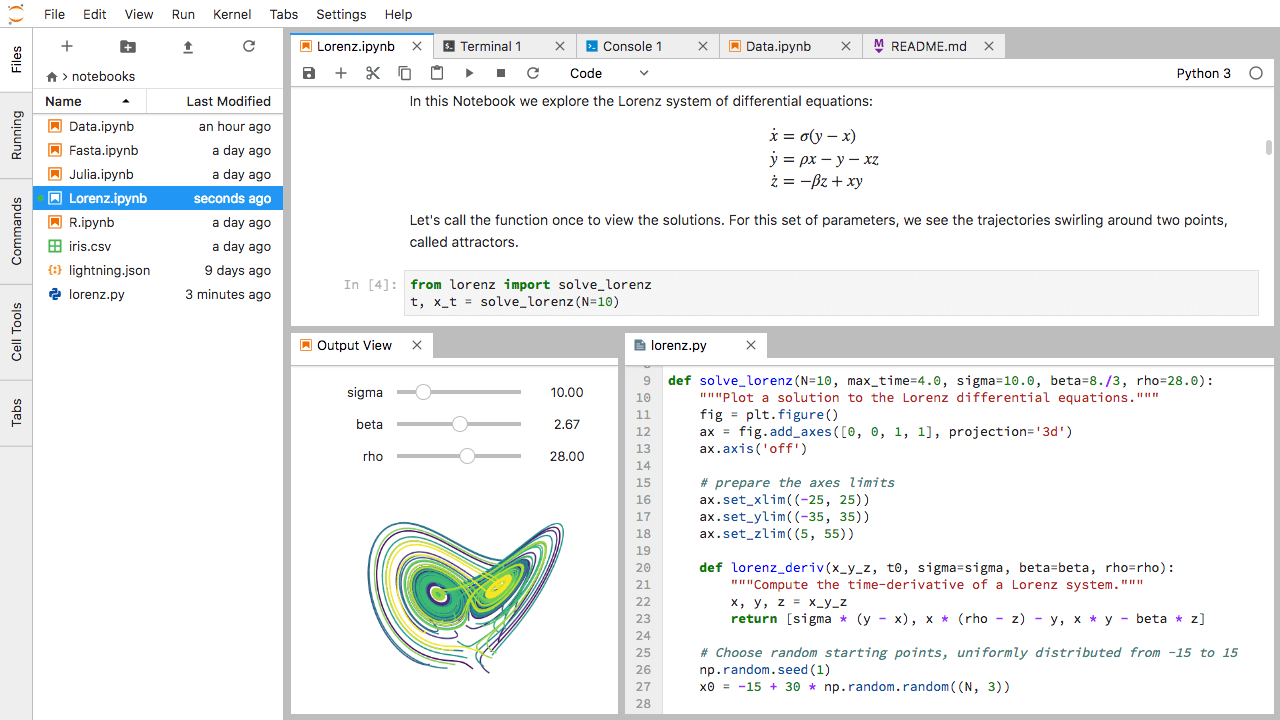
\includegraphics[width=0.95\linewidth]{jupyterlab.png}
%% \end{frame}

%% \begin{frame}{Scikit-Learn and other machine learning tools}
%% \vspace{0.5 cm}
%% SciPy has extensible ``\href{https://www.scipy.org/scikits.html}{\textcolor{blue}{scikits}}'' for specific domains: machine learning is one of these.

%% \vspace{0.25 cm}
%% \uncover<2->{In 2012 (ancient history), Scikit-Learn unified classic machine learning algorithms in one package. (R users had to remember things like ``for Na\"ive Bayes, import e1071.'')}

%% \vspace{0.25 cm}
%% \begin{uncoverenv}<3->
%% Rapid development in deep learning: proliferation of tools, not as unified anymore.

%% \vspace{0.15 cm}
%% \mbox{ } 
\includegraphics[height=0.8 cm]{sklearn-logo.png}
%% \hfill 
\includegraphics[height=0.8 cm]{pytorch-logo.png}
%% \hfill 
\includegraphics[height=0.8 cm]{keras-logo.png}
%% \hfill 
\includegraphics[height=1 cm]{tensorflow-logo.png}
%% \hfill 
\includegraphics[height=0.8 cm]{caffe2-logo.png}
%% \hfill 
\includegraphics[height=0.8 cm]{gluon-logo.png} \mbox{ }

%% \vspace{0.15 cm}
%% \mbox{ } 
\includegraphics[height=0.8 cm]{chainer-logo.png}
%% \hfill 
\includegraphics[height=0.8 cm]{cntk-logo.png}
%% \hfill 
\includegraphics[height=0.8 cm]{lasagne-logo.png}
%% \hfill 
\includegraphics[height=0.8 cm]{onnx-logo.png}
%% \hfill 
\includegraphics[height=0.8 cm]{cesium-logo.png}
%% \hfill 
\includegraphics[height=0.8 cm]{xgboost-logo.png} \mbox{ }
%% \end{uncoverenv}

%% \vspace{0.5 cm}
%% \begin{uncoverenv}<4->
%% \small
%% \textcolor{darkblue}{Questions (show of hands):}
%% \vspace{-0.2 cm}
%% \begin{enumerate}\setlength{\itemsep}{-0.1 cm}
%% \item Who has used a machine learning package in Python (not TMVA)?
%% \item Who has used TMVA (in ROOT, possibly through PyROOT)?
%% \item Who hasn't?
%% \end{enumerate}
%% \end{uncoverenv}
%% \end{frame}

%% \begin{frame}{Scientific Python ecosystem is lacking some tools for HEP}
%% \vspace{-0.5 cm}
%% \begin{columns}[t]
%% \column{0.5\linewidth}
%% \begin{center}
%% \textcolor{darkblue}{\underline{\large What we can find off-the-shelf}}

%% \vspace{0.18 cm}
%% fast data sharing with C/C++

%% \vspace{0.18 cm}
%% fast calculations of user functions

%% \vspace{0.18 cm}
%% libraries of special functions, matrix math

%% \vspace{0.18 cm}
%% fitting/minimization, integration, differentiation, interpolation

%% \vspace{0.18 cm}
%% symbolic algebra

%% \vspace{0.18 cm}
%% advanced statistics

%% \vspace{0.18 cm}
%% machine learning

%% \vspace{0.18 cm}
%% graphics, advanced plotting

%% \vspace{0.18 cm}
%% graphical interfaces, user workflows

%% \vspace{0.18 cm}
%% parallel and distributed processing
%% \end{center}

%% \column{0.5\linewidth}
%% \begin{center}
%% \textcolor{darkblue}{\underline{\large What we must develop in-house}}

%% \vspace{0.18 cm}
%% reading/writing ROOT files

%% \vspace{0.18 cm}
%% integration with collaboration frameworks

%% \vspace{0.18 cm}
%% advanced histogramming

%% \vspace{0.18 cm}
%% efficient variable-length lists \\ (e.g.\ number of electrons per event)

%% \vspace{0.18 cm}
%% HEP functions (e.g.\ boost 4-vectors)

%% \vspace{0.18 cm}
%% HEP-style limit setting
%% \end{center}
%% \end{columns}
%% \end{frame}

%% \begin{frame}{Prepared notebooks: things we can talk about}
%% \vspace{0.3 cm}
%% \renewcommand{\arraystretch}{1.1}

%% \begin{tabular}{p{0.45\linewidth} >{\centering\arraybackslash}p{0.15\linewidth} p{0.3\linewidth}}
%% \textcolor{darkorange}{\bf Scientific Python software} & \textcolor{darkorange}{\bf install} & \textcolor{darkorange}{\bf tutorial} \\\hline
%% Numpy & pip & numpy.ipynb \\
%% Pandas & pip & pandas.ipynb \\
%% Numba and Cython (code acceleration) & pip & numba-cython.ipynb \\
%% SymPy (symbolic algebra) & pip & sympy.ipynb \\
%% \end{tabular}

%% \vspace{0.25 cm}

%% \begin{tabular}{p{0.45\linewidth} >{\centering\arraybackslash}p{0.15\linewidth} p{0.3\linewidth}}
%% \textcolor{darkorange}{\bf HEP-specific software} & \textcolor{darkorange}{\bf install} & \textcolor{darkorange}{\bf tutorial} \\\hline
%% \sout{PyROOT} & \sout{ROOT} & \sout{May 23} \\
%% \sout{heppy and the like} & \sout{CMSSW} & {\it\scriptsize\sout{(I don't know them well enough)}} \\
%% \textcolor{red}{$^*$}uproot (ROOT $\to$ Numpy) & pip & uproot.ipynb \\
%% \textcolor{red}{$^*$}histbook (histogramming) & pip & histbook.ipynb \\
%% \textcolor{red}{$^*$}OAMap (variable-length lists) & pip & oamap.ipynb \\
%% iminuit (fitting) & pip & iminuit.ipynb \\
%% GooFit (RooFit replacement) & pip & goofit.ipynb \\
%% numpythia (Monte Carlo) & pip & numpythia.ipynb \\
%% \end{tabular}

%% \vspace{-3 cm}
%% \hfill \tiny\textcolor{red}{$^*$made by me\hspace{-0.5 cm}}
%% \vspace{3 cm}
%% \end{frame}

\end{document}
